\chapter{Testing Framework}
Im folgenden Kapitel werden wir auf die einzelnen Komponenten des von uns entwickelten Test Frameworks eingehen und die Funktionsweise erläutern. Die Aufgabe des Test Framework liegt darin, die verschiedenen Prototypen, welche im Laufe dieser Semesterarbeit entwickelt wurden, mit dieses Framework einheitlich testen zu lassen. Das Test Framework wurde parallel zum RMIOnly- Systems mit Concurrency Control entwickelt.

\subsection{Konzept}
Das Framework lässt sich über eine Konfigurationsdatei konfigurieren und kann Testfälle die in einer XML Datenstruktur vorliegen intepretieren und daraus die einzelnen Testszenarien generieren. Die Testszenarien werden vom Server auf die verfügbaren Testframework Clients verteilen und dort gestartet. Das Framework startet das zu testende System auf den verschiedenen Rechnern und führt die im XML beschriebenen Szenarien durch.\newline
Die mit den Messwerten ausgefüllten Szenarien werden an den Server zurückgeschickt und dort ausgewertet. Dies ermöglicht ein Vergleichen der verschiedenen eingesetzten Algorithmen. Folgende Eckpunkte muss das Framework erfüllen:

\begin{itemize}
\item Die enwickelten Systeme müssen sich ohne Programmcode-Anpassungen an das Framework anbinden lassen
\item Das Framework muss die genauen Zeiten, welche für die Ausführungen der Operationen nötig waren, messen können
\item Nach einem Testlauf muss ein Bericht erstellt werden können, welcher die nötigen Informationen darstellt

\subsection{Open Points (TODO's)}
\begin{itemize}	
\item Netzwerk Traffic der im Zimmer Auftritt kann nicht kontrolliert werden. Messungen daher nicht verlässlich, man bäuchte ein eigenes Netz.
\item JVM Profiler: Beweis für die Zombie Objekte in der JVM, soll das gemacht werden?
\item Exception Handling
\end{itemize}


\subsection{Der Frameworkserver}
\label{sec:test-FW Server}
\subsubsection{Das Startup-Script}
\label{sec:startupScript}
Das  Startup-Script ist ein Shell-Script in der Bash-Sprache geschrieben. Das Script führt mehrere Methoden nacheinander aus:
\begin{enumerate}
\item Das Script prüft die in der Config-Datei eingetragenen Zielrechner auf bereits vorhandene "client.jar"-Dateien und löscht diese Dateien, falls vorhanden
\item Durch die Applikation "Secure Copy" wird die zuvor im Buildprozess erstellte Datei "client.jar" auf die Zielrechner kopiert
\item Via SSH wird der Frameworkclient auf den Zielrechnern gestartet
\item Der Frameworkserver wird gestartet
\end{enumerate}
Sind diese Schritte abgeschlossen, beendet das Startupscript und die weitere Ausführung des Testlaufs wird durch den Frameworkserver orchestriert.
Beim Starten des Scripts wird der Name der Datei mitgegeben, in welcher der genaue Testlauf definiert ist. Wird kein Argument mitgegeben, läuft der Standardtestlauf ab, welcher in der Datei "testCases.xml" beschrieben ist.
Probleme beim Schreiben des Scripts waren selten. Ein Problem, welches gelöst werden musste war der Umstand, dass das Script nach dem Starten eines Clients nicht mehr weiterlief, sondern einfach wartete. Dies war bei folgende Zeile der Fall:
\begin{lstlisting}	
 ssh student@${i} "java -jar ${remotePath}/${clientJar}"
\end{lstlisting}	
Offensichtlich wartet das Script beim Ausführen eines Befehls auf einem fremden Rechner auf einen Rückgabewert in irgendeiner Form; also auf einen Errorcode oder aber auf einen Exitstatus. Das Absetzen dieses Befehls musste also in einem seperaten Kind-Prozess stattfinden, damit der Eltern-Prozess die weiteren Aufgaben des Scripts abarbeiten konnte und nicht auf einen Rückgabewert wartete. Dies kann in der Bash-Shell mit einem "\&" erreicht werden. Die simple Lösung des Problems sieht also fast gleich aus:
\begin{lstlisting}
 ssh student@${i} "java -jar ${remotePath}/${clientJar}" &
\end{lstlisting}

\subsubsection{Startprozess des Frameworkservers}
\label{sec:startFramework}
In diesem Kapitel werden die Schritte beschrieben, welche vor dem Starten des Testlaufs durchgeführt werden. Der Frameworkserver, einmal gestartet, administriert den ganzen weiteren Ablauf des Testlaufs. \newline
Die Kommunikation des Frameworkservers mit den Frameworkclients ist in folgendem Sequenzdiagramm grob dargestellt:

\begin{center}
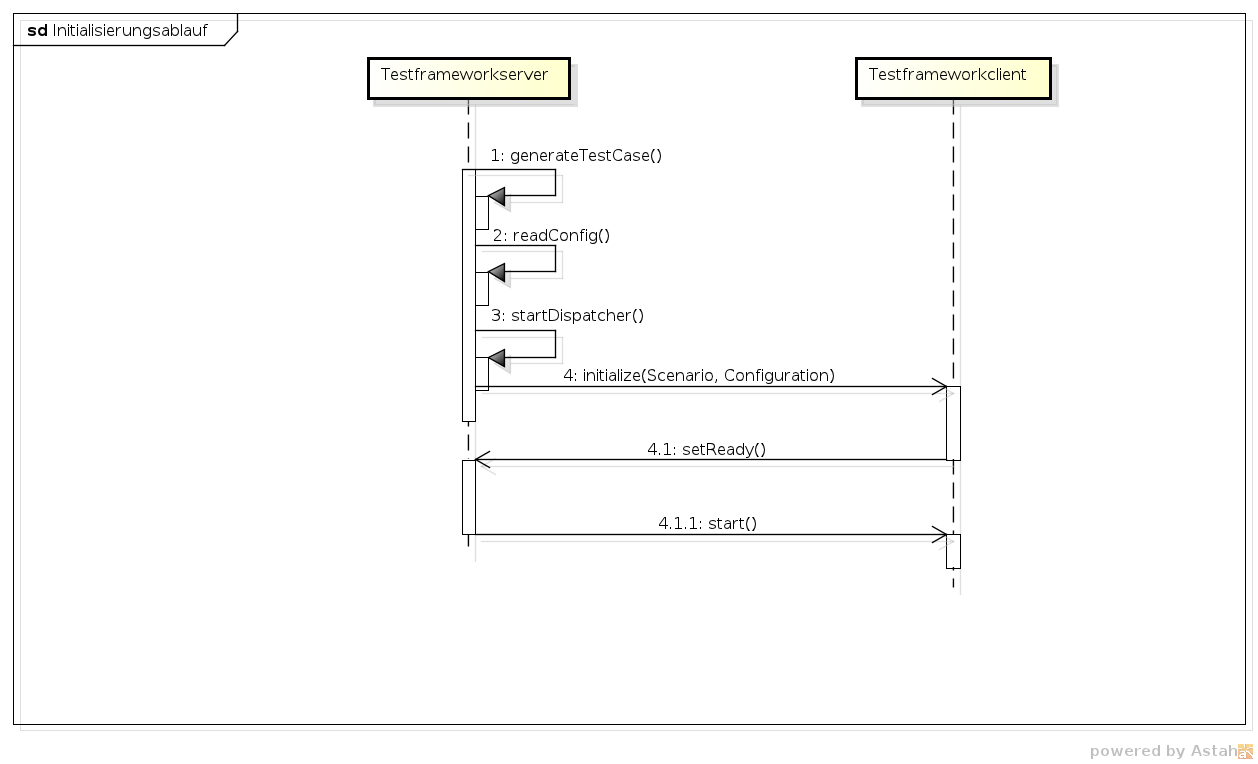
\includegraphics[scale=0.3]{image_testFramework/TestFWInit.png}
\end{center}

Die im Diagramm dargestellten Operationen lassen sich wie folgt erklären:

\begin{itemize}
\item Die Methode generateTestCase() ruft eine Factory auf, welche aus einer XML-Datei einen Testcase generiert. Diese Factory wird unter dem Kapitel Testcase-Factory genauer beschrieben.
\item Alle Konfigurationsparameter welche der Server braucht, sind in einer Konfigurationsdatei abgelegt. Durch eine Configurationfactory wird durch mit Hilfe der Konfigurationsdatei ein Configuration-Objekt erzeugt. Unter dem Kapitel "Configuration-Factory" wird dies näher beschrieben.
\item Nachdem die Konfigurationsparameter ausgelesen wurden, kann der Dispatcher in einem seperaten Thread gestartet werden. Weitere Ausführungen sind unter dem Kapitel "Der Dispatcher" zu finden.
\item Bei der Initialisierung der Clients, wird diesen je ein Scenario und ein Configuration-Objekt gesendet. Das Configuration-Objekt umfasst alle für den Client wichtigen Konfigurationsparameter, wie etwa die Ports, unter welchen der Server seine Dienste zur Verfügung stellt. Was ein Scenario genau ist wird unter dem "Kapitel Testcase-Factory" genauer beschrieben.
\item Pro Client hat der Server beim Auslesen der Konfigurationsdatei ein Client-Objekt instanziert. Dies wurde vorallem zur Kontrolle der Clients durch den Server so implementiert. Darauf wird im Kapitel "ClientObjekt" eingegangen.
\item Nachdem alle Clients "setReady()" aufgerufen haben, ruft der Server "start()" auf allen Clients auf. Dieser Vorgang wird unter dem Punkt "die Start-Methode" genauer erläutert.
\end{itemize}

\subsubsection{Testcase-Factory}
\label{sec:testCaseFactory}
Die Testcase-Factory liest ein XML-File, in welchem ein sogenannter "TestCase" definiert ist. Wird beim Starten des Frameworkservers kein Paramter mitgegeben, wird der Standard-Testcase gewählt, welcher in der Datei "testCases.xml" abgelegt ist. Wird aber ein Parameter mitgegeben, beschreibt dieser den Namen der auszuführenden TestCase-Datei.\newline
Durch die eingelesenen Informationen erstellt die Factory die Szenarien, welche dann weiter an die verschiedenen Clients gesendet werden. Folgender Block ist ein Auszug aus einer TestCase-Datei:

\begin{lstlisting}[language=XML, breaklines=true] 	
<?xml version='1.0' encoding='UTF-8'?>
<TestRun>
  <TestCase SystemUnderTest="ch.hsr.objectCaching.rmiOnlyClient.RMIonlyClientSystem">
    <Account balance="1"></Account>
      <Scenario id="1">
        <ActionSequence>
          <Increment count ="100" delay="0" factor="1.1"></Increment>
	</ActionSequence>
      </Scenario>
      <Scenario id="2">
	<ActionSequence>
          <Increment count ="100" delay="0" factor="1.1"></Increment>
	</ActionSequence>
      </Scenario>
  </TestCase>
</TestRun>
\end{lstlisting}

Das Attribut "SystemUnderTest" definiert das zu testende System. Der Vorteil dieser Methode ist, dass das zu testende System einfach in XML angegeben wird und dann getestet werden kann. Es müssen also keine Anpassungen am Code vorgenommen werden, egal welches System getestet werden soll. Dem Framework ist es schlussendlich egal, welches System getestet werden soll.\newline
Eine TestCase-Datei beschreibt genau einen TestCase. Ein TestCase kann verschiedene Szenarien beinhalten, oder aber auch nur ein Szenario beschreiben. Ist nur ein Szenario definiert, werden beide Clients mit demselben Szenario arbeiten. Falls mehrere Szenarien beschrieben sind, werden die Clients unterschiedliche Szenarien durchführen. \newline
Aus obigem XML-Code generiert die Factory nun ein Objekt vom Typ TestCase. Dieses Objekt definiert nun zwei Szenarien, welche wiederum aus mehreren Actions bestehen. Was genau eine Action ist, ist unter dem Kapitel "Actions" beschrieben. Die Factory wird nun bei diesem Beispielcode eine Abfolge von 100 "Increment-Action" erstellen und diese in das Scenario-Objekt ablegen.


\subsubsection{Configuration-Factory}
\label{sec:configurationFactory}
Die Configuration-Factory liest alle Daten aus der Konfigurationsdatei aus und erstellt mit diesen Informationen ein Configuration-Objekt. Die Konfigurationsdatei sieht wie folgt aus:
\begin{lstlisting}
Client0=152.96.193.18
Client1=152.96.193.19
Clientport=36927
ServerRmiPort=36925
ServerSocketPort=36926
ServerRegistryName=Server
ClientRegistryName=Client
\end{lstlisting}

In der Konfigurationsdatei ist definiert, welche Clients auf welchem port kontaktiert werden können. Weiter ist der Registry-Name definiert, damit der Server weiss, über welche Registry er die Methoden auf dem Client aufrufen muss. \newline
Auf diesen Informationen erstellt die Factory ein Configuration-Objekt, welches sie dem Client als erstes sendet. Damit ist gewährleistet, dass der Frameworkserver und die Frameworkclients miteinander über RMI kommunizieren können. \newline
Pro Client, welcher hier definiert ist, wird ein Client-Objekt instanziert, was im folgenden Kapitel beschrieben wird.

\subsubsection{ClientObjekt}
\label{sec:ClientObjekt}

Das Clientobjekt besitzt unter anderem ein Datenfeld, welches genau zwei Zustände annehmen kann: Ready und NotReady. Führt der Frameworkclient die Methode "setReady()" auf dem Server aus, wird der Status auf dem jeweiligen Objekt auf Ready gesetzt. Folgend die Implementation der setReady-Methode:
\begin{lstlisting}
public void setReady(String ip) 
{
	logger.info("Setted ready with: " + ip);
	Client temp;
	if((temp = clientList.getClientByIp(ip)) != null)
	{
		temp.setStartingState(StartingState.READY);
	}
	if(checkAllReady())
	{
		start();
	}
}
\end{lstlisting}

Interessant an dieser Methode ist die Funktion der "checkAllReady"-Methode. Dieser Mechanismus ist nicht nur dazu da, um alle Clients möglichst gleichzeitig zu starten, sondern auch, um die Threads zu steuern. Die Methode setReady() wird durch mehrere verschiedene Threads aufgerufen, von jedem Client genau ein Mal. Durch die Implementation von checkAllReady() wird aber nur der letzte Thread, welcher setReady() aufruft, weiterleben und start() ausführen können. Somit ist garantiert, dass auch danach nur ein Thread aktiv ist und keine Seiteneffekte entstehen können.\newline
Die Implementation dieser Logik war nicht schwer, doch das Bewusstsein für die Problematik mit mehreren Threads muss ständig vorhanden sein. Die Einflüsse der parallelen Programmierung stellten ohnehin einen spannenden Aspekt dieser Arbeit dar. 

\subsubsection{Die Start-Methode}
\label{sec:startMethode}

Die Methode "start()", gibt dem Client an, mit der Abarbeitung des Szenarios zu beginnen. Die erste Implementation dieser Methode sah wie folgt aus:
\begin{lstlisting}
private void start()
{
	logger.info("Method start() invoked");
	for(int i = 0; i < clientList.size(); i++)
	{
		clientList.getClient(i).getClientStub().startTest();
	}
}
\end{lstlisting}

Nach einigen Testdurchläufen konnte festgestellt werden, dass die Clients ihre Szenarien nur sequentiell abarbeiteten und die Operationen auf den Server nicht gleichzeitig geschehen. Schuld an diesem Umstand war obige Implementation der "start"-Methode. Der Server-Thread, welcher "startTest()" auf dem Client aufrief, wartete solange, bis die Methode zurückkehrte. Da die Methode natürlich erst nach der Beendigung des Szenarios zurückkehrt, konnte nur immer genau ein Client zu einem gewissen zeitpunkt aktiv sein.\newline
Die jetzige Implementation und somit die Lösung des Problems sieht wie folgt aus:
\begin{lstlisting}
private void start()
{
	logger.info("Method start() invoked");
	for(int i = 0; i < clientList.size(); i++)
	{
		ClientStart clientStart = new ClientStart(clientList.getClient(i));
		new Thread(clientStart).start();
	}
}
\end{lstlisting}
Um das Problem mit der Erstellung eines neuen Threads für jeden zu startenden Client zu umgehen, musste eine weitere Klasse Namens ClientStart geschrieben werden. Die Klasse implementiert natürlich das Interface "Runnable" und implementiert die "run()"-Methode wie folgt:
\begin{lstlisting}
public void run() {
	try {
		client.getClientStub().startTest();
	} catch (RemoteException e) {
		logger.log(Level.SEVERE, "Uncaught exception", e);
	}
}
\end{lstlisting}

Mit dieser Implementation wird der Methodenaufruf "start()" nun von einem seperaten Thread ausgeführt. Dies führt dazu, dass die Clients nun zeitlich parallel gestartet werden und nicht nacheinander. Da die einzelnen Threads nach Beendigung der "run()"-Methode sterben, ist die Art der Implementation unbedenklich bezüglich Seiteneffekte oder "zombie-Threads".

\subsubsection{Der Dispatcher}
\label{sec:dispatcher}

Der Dispatcher stellt die Verbindung zwischen dem Frameworkserver und dem Server des Systems, welches getestet werden soll, dar. Dem Dispatcher wird die Portnummer angegeben, unter welcher ein Socket öffnen soll. Weiter wird ihm ein String übergeben, in welchem der Pfad des zu testenden Systems drinnsteht. Der Dispatcher instanziert dann das zu testende System mit Hilfe des Strings und wartet dann in einem blockierten Zustand auf sich verbindende Clients. Nachdem ein Client auf dem geöffneten Socket eine Verbindung aufgebaut hat, übergibt der Dispatcher die Verbindung in Form eines Input und eines Outputstreams dem Server des zu testenden Systems.\newline
Logischerweise läuft der Dispatcher wiederum in einem seperaten Thread.

\subsubsection{Herunterfahren des Frameworkservers}
\label{sec:herunterfahrenFramework}

Nach Beendigung eines Testlaufs, muss der Server mehrere Arbeiten erledigen. Nachfolgend werden die wichtigsten Aufgaben, welche der Server nach einem Testlauf erledigen muss, aufgeführt:

\begin{center}
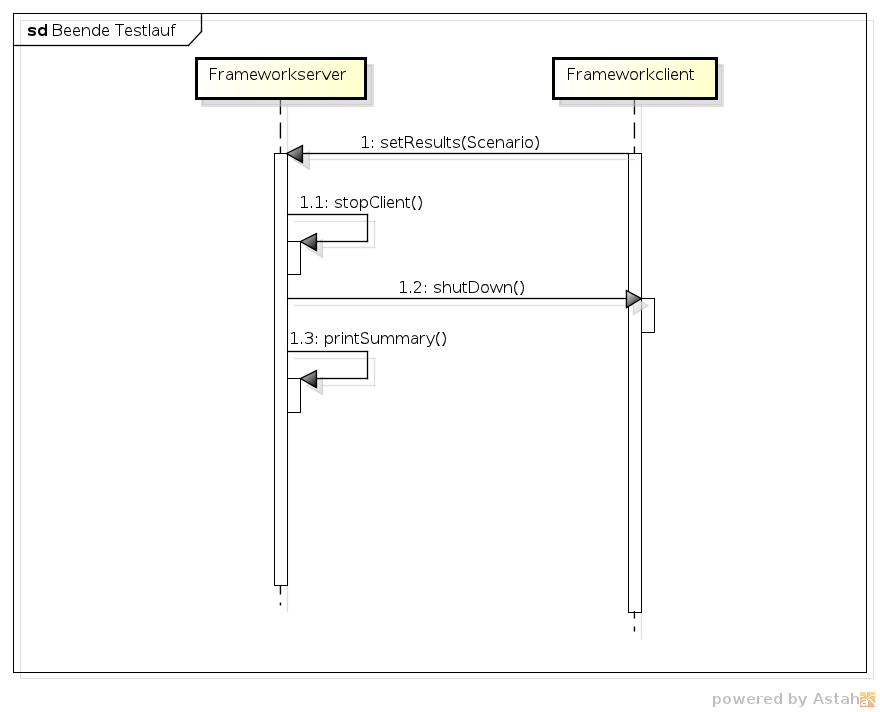
\includegraphics[scale=0.2]{image_testFramework/BeendeTestlauf.png}
\end{center}

Die im Diagramm ersichtlichen Operationen können folgendermassen erläutert werden:
\begin{itemize}
\item Die Methode "setResults(Scenario)" wird vom Client auf dem Server aufgerufen. Durch den Aufruf dieser Methode weiss der Server, dass der aufrufende Client sein Szenario durchgespielt hat. Weiter wird mit dem Aufruf der Methode wiederum ein Thread durch den RMI-Daemon gestartet, welcher die weiter folgenden Methoden anstösst.
\item Aus der "setResults(Scenario)"-Methode wird direkt "stopClient()" aufgerufen. Was diese Methode genau macht, wird im Kapitel "Stoppen eines Clients" genau beschrieben.
\item Die Methode "shutDown()" wird auf dem Client aufgerufen. Der Client trennt daraufhin die RMI-Verbindung zum Server und schaltet sich selber ab. Nähere Informationen zum Abschaltungsprozess eines Clients kann unter dem Kapitel "Testframework Client" nachgelesen werden.
\item Die Methode "printSummary()" verwertet die Ergebnisse, welche die CLients in ihrem Szenario gespeichert und wieder übertragen haben. Mehr Informationen dazu im Kapitel "Report Generator". Weiter wird auf der Console ausgegeben, ob es "Lost-Update"-Probleme gegeben hat oder nicht. Mehr zu diesem Thema unter "Result Generator".
\end{itemize}

\subsubsection{Stoppen eines Clients}
\label{sec:stopClient}
Ruft ein Client die Methode "setResults(Scenario)" auf dem Server auf, wird Serverintern der Status des Clients auf "Down" gesetzt. Da die Methode "stopClient()" wiederum pro Client genau ein Mal aufgerufen wird, entsteht wieder das Problem, dass mehrere Threads am Leben sind. Um dies ab einem gewissen Punkt zu verhindern, wurde ähnlich zur "setReady()"-Methode, folgende Implementation gewählt:
\begin{lstlisting}
private void stopClient(String clientIp)
{
	Client temp;
	try {
		
		if((temp = clientList.getClientByIp(clientIp)) != null)
		{
			logger.info("stop client with ip: " + clientIp);
			temp.setClientRunning(ShutedDown.DOWN);
			temp.getClientStub().shutdown();
		}
	} catch (RemoteException e) {
		logger.log(Level.SEVERE, "Uncaught exception", e);
	}
	if(checkAllShutedDown())
	{
		printSummary();
	}
}
\end{lstlisting}

Durch die Prüfung "checkAllShutedDown()", wird nur der letzte aller Threads weiterleben. Somit wird auch nur ein Thread fähig sein die Methode "printSummary()" auszuführen, während die anderen Threads die Methode zu Ende abarbeiten und am Ende der Methode sterben. Durch diese Implementation wird sichergestellt, dass nur ein Thread weiterlebt und keine "Zombi-Prozesse" mehr vorhanden sind.\newline
Weiter wird beim Abarbeiten dieser Methode die Methode "shutdown()" auf dem Client aufgerufen. Nach diesem Aufruf fährt sich der Client herunter und kappt alle akiven Verbindungen zum Server. Weitere Informationen zum Shutdown-Prozess des Clients sind unter der Kapitel des Frameworkclients ersichtlich.

\subsubsection{Report Generator}
\label{sec:reportGenerator}

Wir die Methode "printSummary" aufgerufen, wird ein ReportGenerator instanziert, welche die Daten der Clients ausliest und in eine Textdatei schreibt. Folgende Werte wurden durch die Clients erfasst:
\begin{itemize}
\item Zeit, welche benötigt wurde um die entsprechende Action durchzuführen
\item Protokollierung, ob bei der Durchführung ein Konflikt generiert wurde oder nicht
\item Zeit, welche in einem Konfliktfall gebraucht wurde, um den Konflikt zu behandeln und die Operation noch einmal auszuführen
\end{itemize}

Pro Client wird eine Datei erstellt, in welcher die Daten dargestellt werden. Folgend einen kurzen Auszug eines solchen Reports:

\begin{lstlisting}
************************************************************
Result for Client: 152.96.193.18 with ScenarioID: 1
OS: Linux / 3.0.0-17-generic-pae
************************************************************
ActionNr;#ofTries;Time[ms];ACTION
0;0;42.674487;INCREMENT(READ) WITHOUT DELAY
0;1;77.969046;INCREMENT(WRITE) WITHOUT DELAY
1;0;79.684003;INCREMENT(READ) WITHOUT DELAY
1;1;81.984427;INCREMENT(WRITE) WITHOUT DELAY

------------------------------------------------
100% of all Action executed are successful
Total actions executed: 2, number of unsuccessful action 0
Total getBalance calls: 2, avg. execution time 61.179245
Total setBalance calls: 2, avg. execution time 79.9767365

Total Conflict: 0 / Gesamt Dauer: 282.311963 ms / durch. Dauer pro Operation: 141.1559815
\end{lstlisting}

Die genaue Messerwerte, mit Durchschnittswerten und Vergleiche zwischen verschiedenen Systemen sind am Schluss dieser Arbeit zu finden.

\subsubsection{Result Generator}
\label{sec:resultGenerator}
Der ResultGenerator ist ein Generator, welcher für die Berechnung des zu erwartenden Entbestandes des Account-Objektes verantwortlich ist. Wenn alle Clients ihre Operationen abgeschlossen haben, wird das aktuelle Ergebnis des Account-Objektes und das erwartete Ergebnis auf der Konsole ausgegeben. Zusätzlich wird kontrolliert, ob die Ergebnisse übereinstimmen und eine entsprechende Meldung wird auf der Konsole ausgegeben:
\begin{lstlisting}
19.04.2012 18:33:38 ch.hsr.objectCaching.testFrameworkServer.Server printSummary
INFO: AccountBalance is: 1.4641001269340557
19.04.2012 18:33:38 ch.hsr.objectCaching.testFrameworkServer.Server printSummary
INFO: AccountBalance should be: 1.4641001269340557
19.04.2012 18:33:38 ch.hsr.objectCaching.testFrameworkServer.Server printSummary
INFO: No Lost-Updates!
\end{lstlisting}

\subsubsection{Logger}
\label{sec:logger}
Wie in dem Konsolenauszug unter "Result Generator" gesehen werden kann, wurde ein Logger eingebaut, welcher alle Methodenaufrufe protokoliert. Der Logger schreibt die Ereignisse erstens auf die Konsole und zweitens schreibt er alle Informaionen zu einem Methodenaufruf in eine Datei. Diese Logdatei ist sehr Informationsreich:

\begin{lstlisting}
<record>
  <date>2012-04-05T17:58:43</date>
  <millis>1333641523151</millis>
  <sequence>9</sequence>
  <logger>TestFrameWorkServer</logger>
  <level>INFO</level>
  <class>ch.hsr.objectCaching.testFrameworkServer.MethodCallLogger</class>
  <method>methodCalled</method>
  <thread>11</thread>
  <message>setBalance got invoked by /152.96.193.9</message>
</record>
<record>
  <date>2012-04-05T17:58:43</date>
  <millis>1333641523198</millis>
  <sequence>10</sequence>
  <logger>TestFrameWorkServer</logger>
  <level>INFO</level>
  <class>ch.hsr.objectCaching.testFrameworkServer.Server</class>
  <method>setResults</method>
  <thread>12</thread>
  <message>Results from scenario 1 setted by 152.96.193.9</message>
</record>
\end{lstlisting}

Die Notwendigkeit zur Implementierung eines Loggers wurde erst während das Projektes erkannt. Durch die vielen verschiedenen aktiven Threads war eine Überprüfung des korrekten Programmablaufs extrem schwierig. Mit der Hilfe des Loggers konnte dieses Problem behoben werden.

\subsection{Testframework Client}
\label{sec:test-FW Client}
Dieses Kapitel beschreibt die Aufgaben der Testframework Client Komponenten und deren Umsetzung. Der Testframework Clients hat zwei Hauptaufgaben, als erstes erzeugt und konfiguriert er das benötigte ClientSystemUnderTest. Zweitens muss er auf einem ClientSystemUnderTest eine gegebens Szenerio abarbeiten können. Die Umsetzung des Testframeworks wurde über das bewährte Client/Server Konzepts realisiert, was zu einer schlanke Lösung auf Seiten des Clients führte. Dadurch lässt sich der Framework Client und das ClientSystemUnderTest direkt vom Framework Server aus konfigurieren und steuern. Ein weiterer Vorteil liegt darin das sich neue Anforderungen jederzeit leicht umsetzen lassen.


\subsubsection{ClientController}
\label{sec:clientController}

\begin{center}
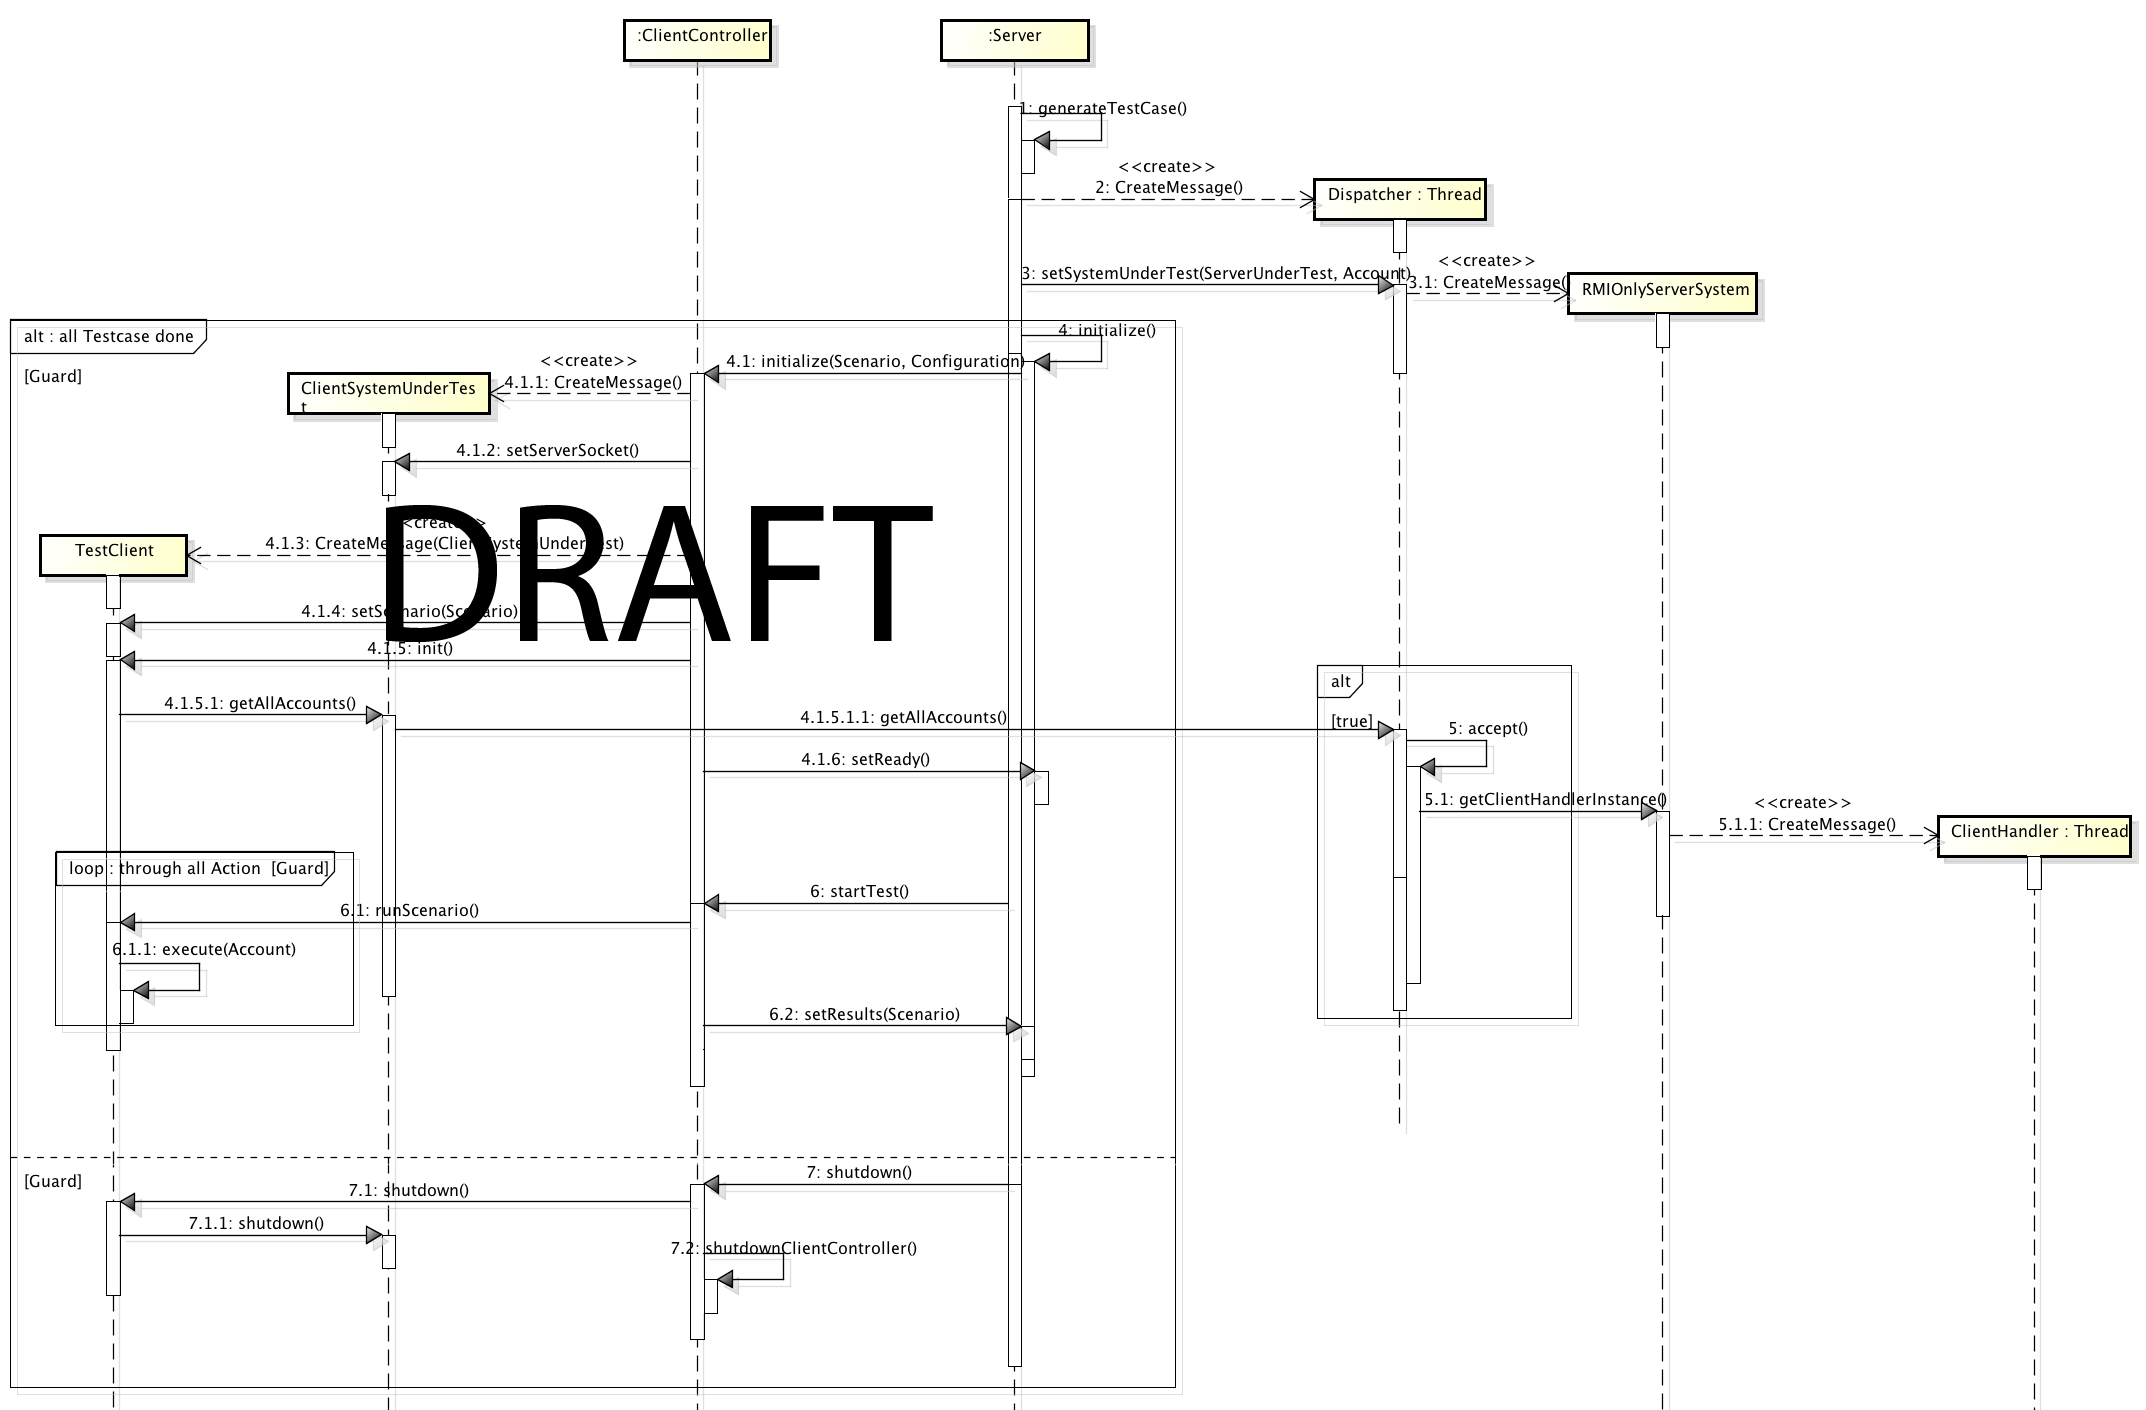
\includegraphics[scale=0.2]{image_testFramework/TestFWServerClientSeq.png}
\end{center}
 
Die Kommunikation zwischen den Testframework Clients und dem Server ist mit Java RMI realisiert worden. Beim Start eines Testframework Clients wird ein neuer ClientController instanziiert, daraufhin wird dieses Objekt zur Java RMI Runtime exportiert. Die Veröffentlichung, das ClientController- Objekts erledigt die RMI Runtime im Hindergrund, ist das Objekt erfolgreich unter dem Namen, der als Argument beim start des ClientController mitgegeben wurde registriert, lässt sich der ClientController über Remote Method Invocation vom Server steuern. Der Port auf der die RMI Registry Anfragen akzeptiert lässt sich ebenfalls via Argument mitgeben falls keine Portnummer als Argument mitgegeben wird, kommt der Defaultport 1099 zum Einsatz.

Folgendes Interface wird vom ClientController implementiert und lässt sich über Java RMI benutzen:
\begin{lstlisting}[language=java, breaklines=true] 	
public void initialize(Scenario scenario, Configuration configuration) throws RemoteException;
public void startTest() throws RemoteException;
public void shutdown() throws RemoteException;
\end{lstlisting}
Über dieses Interface lässt sich der gesamte Testprozess des Clients steuern. Die Idee zu Beginn des Projekts war das alle Konfigurationswete als Parameter an den ClientController übergeben werden. Es stellte sich jedoch schnell heraus, dass die Kappselung alles Parameter in einem seperaten Objekt eine bessere Lösung darstellt. Der Configurationtyp beinhaltet alle nötigen Parameter für die Konfiguration des ClientSystemUnderTest sowie des ClientController. In diesem Objekt ist unter anderem der Namen des ClientSystemUnderTest sowie die nötigen Information für den erfolgreichen Aufbau der RMI Kommunikation zwischen dem Testframework Client und dem Testframework Server. In der initialize() Methode wird als erstes ein Server Stub geladen. Zweitens, wird aus dem Configuration Objekt das gewünschte ClientSystemUnderTest herausgelesen und via Reflection instanziiert. Die Instanziierung des konkreten ClientSystemUnderTest wird in einer seperaten Factory erledigt. Danach wird dem TestClient das erzeugte CUT übergeben. Als letztes wird der TestClient wird mit dem gegeben Szenario initialisiert. Sind alle Vorbereitungsschritte abgeschlossen, wird der Server über die erfolgreiche Initialisierung des CUT und des ClientController informiert. Der Server startet den Testdurchlauf parallel auf allen ClientController über die Methode startTest(). Sind alle Aktionen des gegeben Szenarios abgearbeitet, wird das gesamte Szenario mit den enthaltenen Messresultaten zurück an den Server geschickt, dort wird die Auswertung der Resultate vom Server übernommen. Der Testframework Client sowie das ClientSystemUnderTest laufen in derselben Java Virtual Machine um für jeden Testlauf dieselben JVM Umgebung zu gewährleisten, haben wir uns dazu entschlossen, bei jedem Testcase das ganze System neu zu starten. Über die Methode shutdown() lässt sich daher der Testframework Client sowie der CUT herunterfahren. Die shutdown() Methode löscht das Binding zwischen dem spezifischen Namen und dem damit verbundenen Objekt. Danach wird das Objekt von der RMI Runtime entfernt. Ist dies erledigt beendet sich der ClientController selbst. Beim testen der shutdown() Funktionalität konnte festgestellt werden, dass wenn die Umsetzung des Codes wie oben beschrieben realisiert wurde, dass der Server eine Exception bekommt, dies lag daran das der ClientController zu schnell die Verbindung zum Server beendet hat, so dass der Server keine Zeit fand seine RMI Verbindung zum ClientController korrekt zu schliessen. Die Lösung des Problems lag, in einer kurzen Verzögerung von zwei Sekunden bevor das System sich endgültig beendet. Die Beendigung des ClientController wird in einem seperaten Thread ausgeführt, sodass der main Thread noch genügend Zeit hat, alle offenen Verbindungen ordnungsgemäss zu schliessen.    

\subsubsection{Test Client}
\label{sec:testclient}

\begin{center}
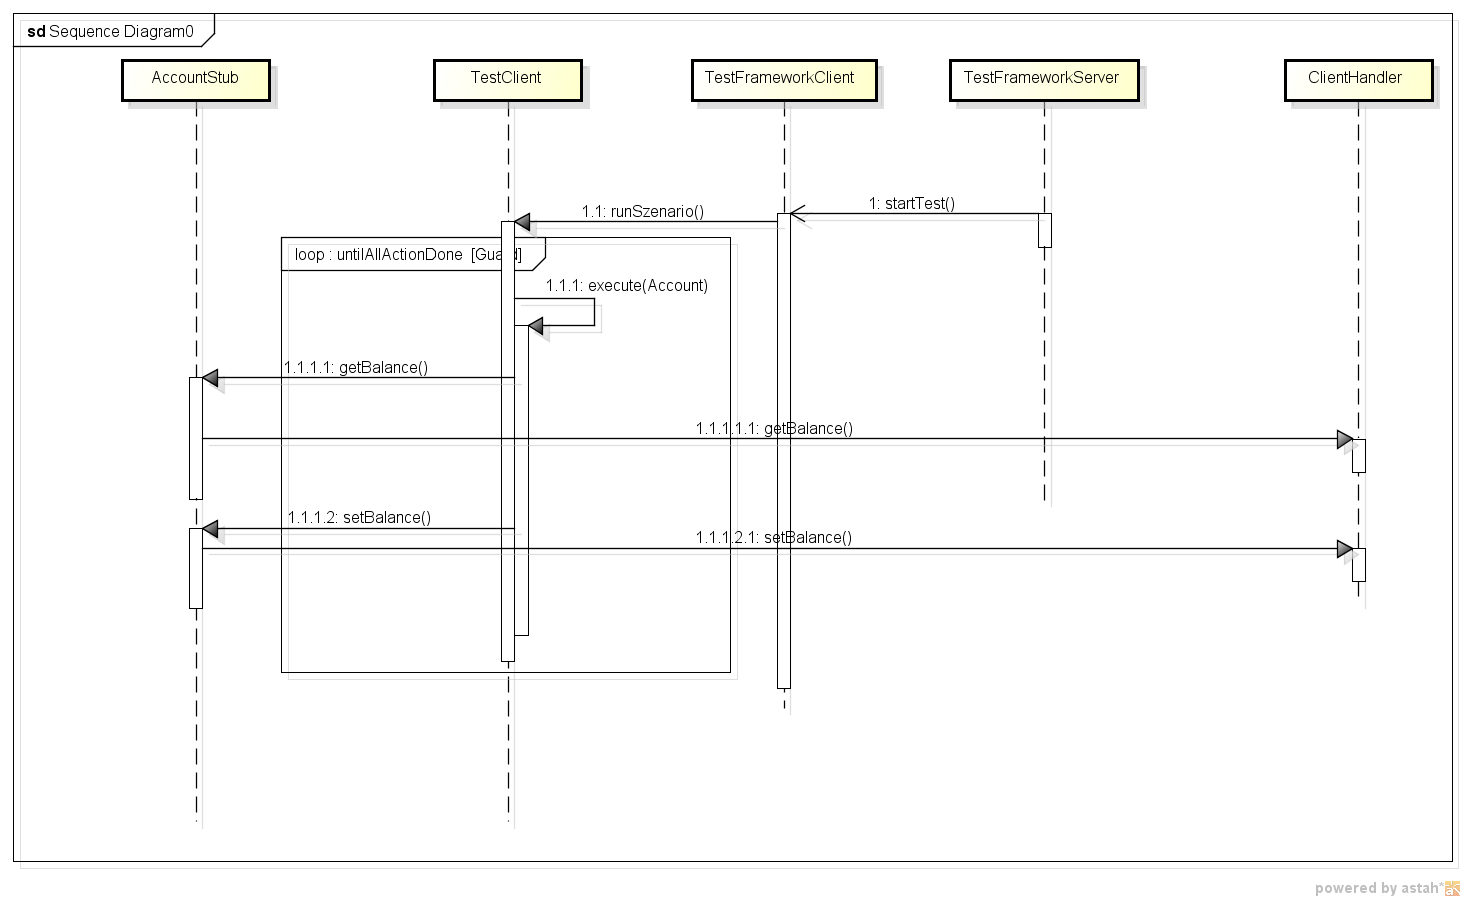
\includegraphics[scale=0.3]{image_testFramework/startTest.png}
\end{center}

Die Klasse TestClient ist die Schnittstelle zwischen dem Testframework und dem ClientSystemUnderTest. Im Konstruktor dieser Klasse kann ein Objekt übergeben werden, welches das ClientSystemUnderTest Interface implementiert. Startet der Server den Testlauf wird im TestClient das zuvor gesetzte Szenario abgearbeitet. Hierfür wird auf jedem Aktion Objekt die Methode execute(Account accunt) aufgerufen. Das Account Objekt, welches der execute Methode übergeben werden muss, wird aus der List von Accounts die von AccountService bereitgestellt wird geholt und übergeben.(Ringbuffer). Bei einem Shutdown durch den Server ist der TestClient ebenfalls für die ordnungsgemässe Beendigung des ClientSystemUnderTest zuständig.

\subsubsection{Action}
\label{sec:action}
Ein Szenario beinhaltet eine Menge von Aktionen die auf ein Account Objekt ausgeführt werden können. Für eine einfache Erweiterbarkeit von neuen Aktionen haben wir hierfür das Command-Pattern genutzt. Alle konkreten Implementierung von Aktionen leiten von der abstrakte Klasse Action ab. Im Konstruktor  dieser abstrakten Klasse wird ein neues Result Objekt instanziert. Dieses Objekt dient als Datenkontainer für alle Zeitmessungen die während dieser Aktion ausgeführt werden sollen. Desweiteren deklariert Action drei abstrakte Methoden die von Subklassen implementiert werden müssen.
\begin{lstlisting}[language=java, breaklines=true] 	
public abstract ActionTyp getActionTyp();
public abstract int getMinimalNumberOfTimeRecords();
public abstract void execute(Account account);	
\end{lstlisting}
Anmerkung: Eine Aktion kann aus mehreren setter/getter bestehen, daher ist es notwendig festzustellen ob die ganze Aktion erfolgreich war oder nicht. Dies wird über die minimale Anzahl von TimeRecords, die für den Erfolg der spezifischen Aktion notwendig sind, gemacht. 


\subsubsection{ActionTyp}
\label{sec:actionTyp}
Der ActionTyp wird zur Indentizifierung der Aktion benutzt und ist als Enum realisiert. Folgende Aktionstypen sind bereits vorhanden.

\begin{itemize}
\item ReadAction
\item WriteAction
\item IncrementAction
\end{itemize}
(Underline im Item funktionieren nicht!!!!)
Die Werte diese Enums werden zur Fallunterscheidung bei der Report Generierung verwendet.

 
\subsubsection{Increment Action}
\label{sec:incrementAction}
Um unsere Anforderungen abdenken zu können, benötigten wir nur die KontoErhöhen Aktion (IncrementAction), die den aktuellen Kontostand des Account Objekts holt (getBalance()) und den aktuellen Kontostand mit dem gegeben Faktor multipliziert und daraufhin den neuen berechneten Kontostand zurück in den Account schreibt(setBalance()). Zusätzlich war es nötig, dass zwischen der der getBalance() und der setBalance() eine minimal definierbare Zeitdauer gewartet werden kann. Diese Warteperiode ist nötig, damit sich leicht ein Konflikt erzeugen lässt und so gezeigt werden kann, dass der Fehler serverseitig zu keinem Lost-Updates führt. Tritt serverseitig ein Concurrency Fehler auf wird eine RuntimeExeption geworfen, dies führt auf der clientseite dazu, dass die ganze Aktion nochmals gestartet wird mit dem Unterschied das diesmal keine Verzögerung zwischen getBalance() und setBalance() vorkommt.

\subsubsection{Result}
\label{sec:result}
Für die Zeitmessung einer Aktion nutzen wir die von Java bereitgestellte Methode System.nanoTime(). Die Result Klasse bietet eine startTimeMeasurement() Methode die ein neues TimeRecord Objekt erzeugt und die momentane Zeit in das TimeRecord Objekt schreibt. (diese Methode verlangt eine BasicAction Typ der als Enum realisiert wurde(Erklärung warum nötig unter Resultate)). Über stopTimeMeasurement() lässt sich die aktuelle Messung beenden und der aktuelle TimeRecord wird abgelegt. Da innerhalb der execute() Methode mehrere setBalance() oder getBalance() möglich sind, muss es möglich sein mehrere TimeRecords pro Result Objekt zu erfassen.

\subsubsection{TimeRecord}
\label{sec:timeRecord}
Der TimeRecordtyp ist als reines Data Tranfer Object ausgelegt. Es beinhaltet die Startzeit sowie die Stopzeit genau einer Aktion. Für einen genauen Auswertung einer Aktion sind noch weiter Daten nötig. Daher besitzt dieser Typ zwei weiter Felder. Der BasicActiontyp beinhaltet Informationen für welche Methode dieser Record gilt und das ActionResult speichert die Information über den Erfolg der BasicAction. Dadurch lassen sich zusammengesetzte Aktion, welche aus getBalance() und setBalance() zusammengesetzt sind unterteilen.

\subsubsection{BasicAction}
\label{sec:BasicAction}
Damit eine genaue Analyse der Aktionen gemacht werden kann, ist es nötig das man unter getBalance() und setBalance() unterscheiden kann. Eine Aktion kann aus mehreren Methodenaufrufen bestehen, daher muss bei einer Zeitmessung die Art(setter / getter) angegeben werden. Da jedoch eine Aktion aus einer Abfolge von Reads und Writes bestehen kann ist es nötig das diese Information gespeichert wird. Im TimeRecord lässt sich daher die BasicAction speichern.

\subsubsection{ActionResult}
\label{sec:ActionResult}
Den Erfolg eines getBalance() oder setBalance() Aufrufs lässt sich ebenfalls im TimeRecord speichern. Um eine Statistik über die Fehlerrate beider Methodenaufrufe zu bekommen, war es desweitern noch nötig, dass beim stoppen einer Messung, der eine BasicAction zugrunde liegt den Erfolgstatus gespeichert werden kann. Damit lässt sich ein Szenario auf die zwei Grundoperation setBalance() und getBalance() herunterbrechen und gibt uns die Möglichkeit eine genau Auswertung der Messresultate zu machen.

\subsubsection{ReportGenerator}
\label{sec:reportGenerator}
Der ReportGenerator analyisiert ein Szenario und schreibt die Resultate in eine Txt-Datei, welche alle relevanten Information beinhaltet. Wir haben uns für eine Textdatei entschieden, da ein Textfile leicht lesbar ist(Grund???). Folgende Messdaten müssen aus einem Report ersichtlicht sein:
\begin{itemize}
\item durchschnittliche Dauer des Methodenaufrufs getBalance()
\item durchschnittliche Dauer des Methodenaufrufs setBalance()
\item Anzahl aufgetretene Konflikte
\item Dauer eines setBalance(); Methodenaufrufs im Falle einer Konfliktsituation
  \begin{itemize}
  \item Zeitdifferenz zwischen erstem setBalance bis erfolgreichem setBalance
  \item Zeitdifferenz zwischen setBalance und Empfang der zugehörigen Exception
  \end{itemize}
\item Dauer des gesamten Szenario
\end{itemize}

Um die obigen Anforderung erfüllen zu können, war es nötig, dass wir unterscheiden können zwischen einer getBalance() und einer setBalance() Aktion, dies wird über den BasicAction-Typ erledigt.
\newline
Die Resultatedatei ist in drei Teile unterteilt. Der erste Teil gibt eine List der Aktionen aus und die dazugehörigen BasicAktion. Über den ActionTyp wird der entsprechende Ausgabestring erzeugt. Es folgt eine Zusammenfassung der zwei BasicAktionarten und zuletzt ein Zusammenfassung über das ganze Szenario.





